\section{合规验证协议}\label{sec:compliance}
根据PFMI\cite{pfmi}的附录四: "支付系统、证券结算系统、中央交易对手的设计纲要",典型的支付过程包括4个环节:
\begin{enumerate}
    \item 收单(Submission): 用户或者代理将支付指令提交给支付系统,指令一般包括发送方账户、接收方账户、额度、签名及其它相关的信息。
    \item 合规性审核(Validation): 接受指令后,支付系统审核支付双方的真实身份,根据所在司法辖区的要求,审核支付的合规性。
    \item 财务性审核(Conditionality): 合规性审核之后,还要通过财务性审核。主要是审核发送方是否有足够的余额,资产是否被冻结等等。
    \item 结算(Settlement): 最后,支付双方的账户完成结算,满足不可撤销性和最终性。
\end{enumerate}

在合规性审核(Validation)环节,金融机构要了解发送方的真实身份、接受方的真实身份,以及交易的背景数据,根据所属司法管辖区的要求审核该交易是否符合金融监管的要求。比如说根据反洗钱法的规定,要收集完整的、真实的、有效的交易背景数据,检查该交易是否涉嫌贩卖毒品、走私贸易、贪污贿赂等非法活动,是否隐瞒资产的来源和性质,试图将其合法化。

但是目前绝大多数分布式账本系统,缺少这种交易前置的手段保证交易的合规性。一般只能在交易之后,分析交易历史记录,追踪非法交易,手段被动而且低效。为了解决这个问题,这一章提出合规验证协议,通过此协议合规机构可以互相协作,验证每一笔交易的合规性。只有合规性检测通过之后,Libra 网络才会接受此交易。

本文只描述合规协议的基本框架和流程,并不是协议的详细规范说明。具体规范会在其它文档中另行说明。

根据第\ref{sec:arrangement}章“组织安排”,合规机构负责管理用户链下的KYC信息,以及审核用户的交易,所以合规审核的主体是合规机构。第\ref{sec:account_structure}章“账户数据结构”,提供了链上的账户与链下的身份管理系统集成方案,以及合规机构服务注册方案。这为合规审核协议提供了基础。

\subsection{典型交易场景}

为了叙述方便,我们先虚拟一个交易场景。不失一般性,假设有两家合规机构,分别为花旗银行(www.citi.com)与摩根大通银行(www.jpmorgan.com)。美国个人和企业可以向这两家合规机构提交真实身份数据,完成账户注册,并且委托他们执行合规审核。
他们的合规系统包括4部分::
\begin{enumerate}
    \item \textbf{KYC}子系统:      存储、管理个人与企业真实身份数据
    \item \textbf{Sanction}子系统: 存储、执行反洗钱(AML) 制裁规则,识别可能的洗钱活动。
    \item \textbf{Repository}子系统: 存储交易记录相关,提升交易透明度。
    \item \textbf{Compliance}子系统: 整合与封装 KYC、Sanction 与 Repository 内部子系统,对外提供合规服务 Rest API 接口,服务的地址保存在对应的 libra.toml 文件中。
\end{enumerate}

为了开展业务,首先他们需要向 Libra 协会实名注册,在 Libra 上建立知名账户,配置域名与 libra.toml文件。

\begin{figure}[h!]
    \centering
    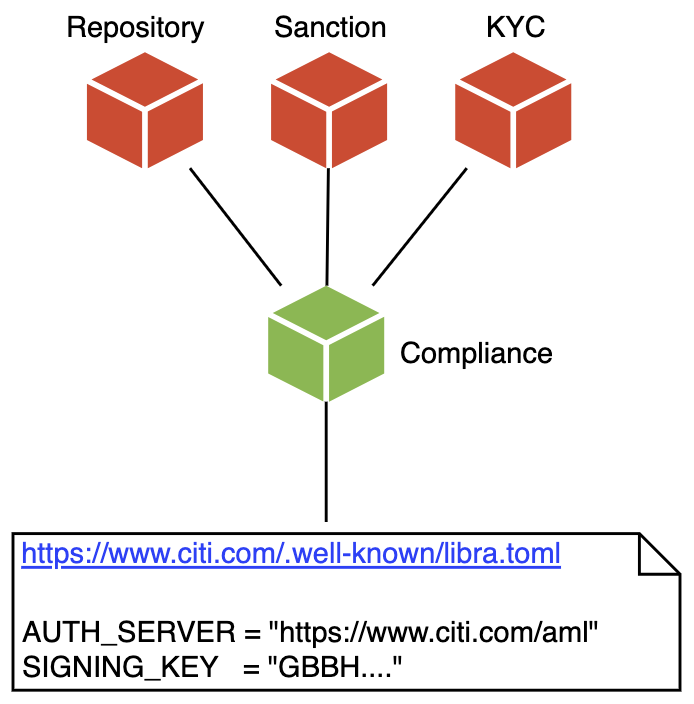
\includegraphics[width=8cm, keepaspectratio]{images/citi.png}
    \caption{花旗银行合规系统架构}
    \label{fig:citi}
\end{figure}


比如在花旗银行的 Libra 账户中,Domain 字段为 \url{www.citi.com},libra.toml 文件的URL为: \url{https://www.citi.com/.well-known/libra.toml}。
如图\ref{fig:citi}所示,其它机构可以通过此文件获取花旗银行的审核服务地址: \url{https://www.citi.com/aml}。

再假设有两个用户:Alice 和 Bob,他们分别向花旗银行与摩根大通银行实名注册,通过KYC审核流程之后,建立 libra 账户。比如,Alice 向花旗银行提交身份相关信息,建立 Libra 账户,账户中的 Validator 的字段是花旗银行的 Libra 账户地址。之后与 Alice 这个账户的所有交易需要花旗的审核通过才能结算。下图\ref{fig:accounts}显示这些账户的关键数据以及彼此之间的关联关系。

\begin{figure}[h!]
    \centering
    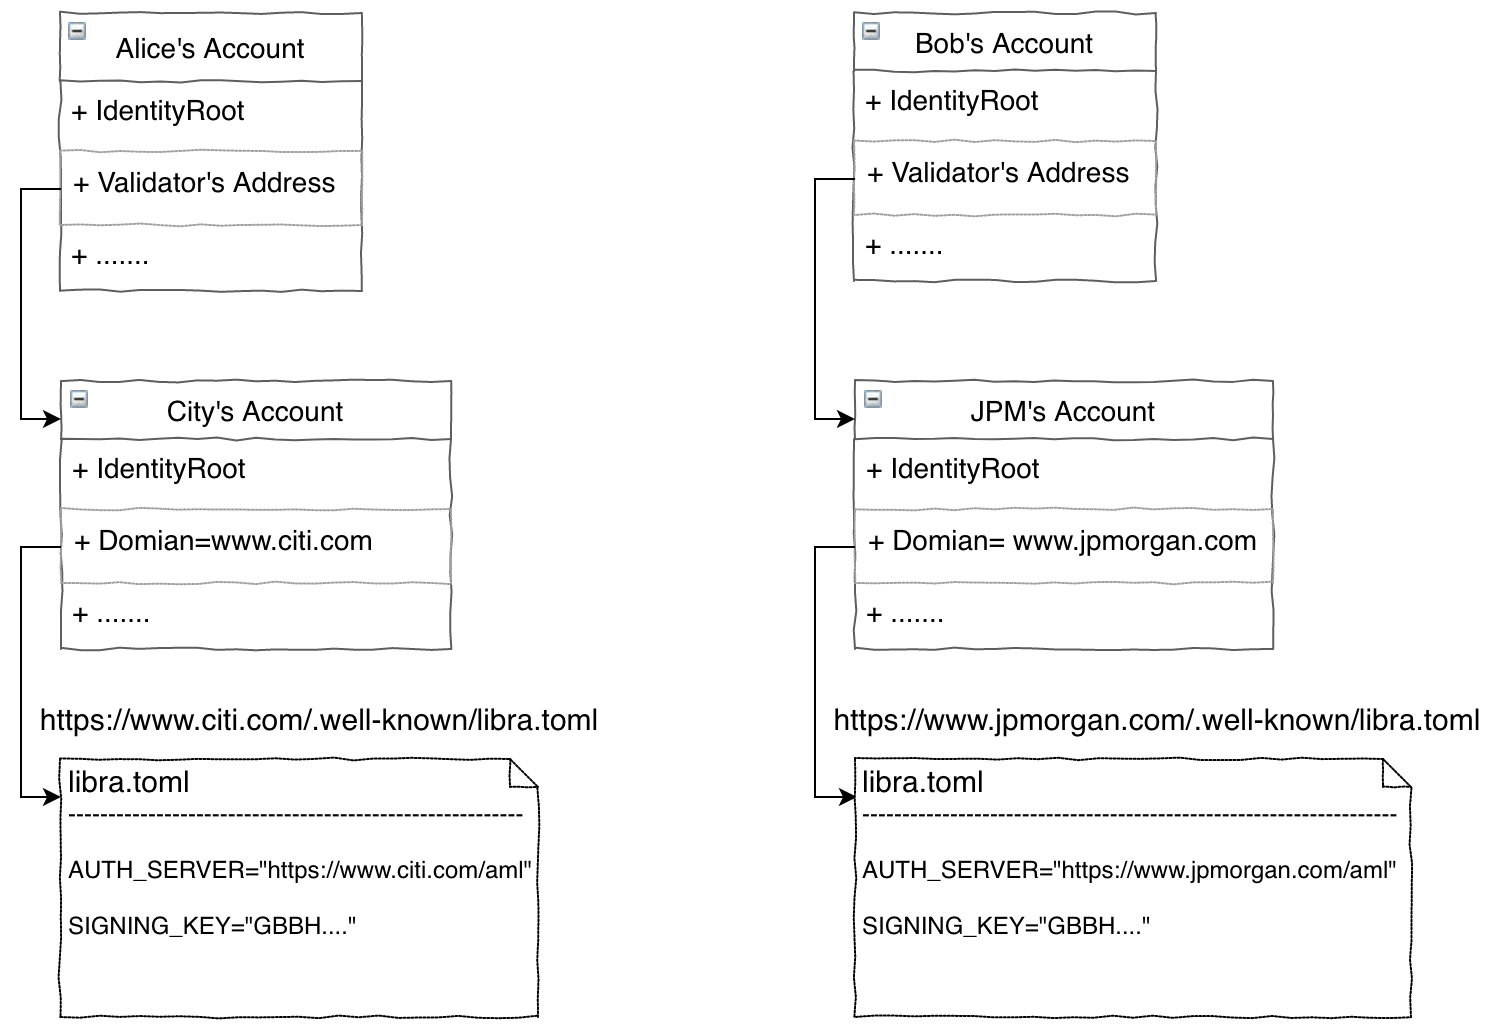
\includegraphics[width=10cm, keepaspectratio]{images/alice_bob.png}
    \caption{Alice、Bob、花旗、摩根大通的Libra账户}
    \label{fig:accounts}
\end{figure}

\subsection{合规审核服务}
每一家合规机构必须公布自己的交易审核服务。此服务根据所在司法辖区的规定,提供AML、CFT等合规审查,审查通过后对交易签名认证。从技术上讲,这是一个 Rest 风格的API服务,对应的服务 URL 地址和签名公钥公布在 libra.toml 文件里。 

%\subsubsection{审核服务消息}

在一个交易被广播到 Libra 网络之前,发送方的合规机构必须向接受方合规机构的审核服务发起请求。
这个请求是一个 HTTP POST 类型的请求,HTTP Header “Content-Type”的值必须为 “application/json”。
请求消息的正文部分是一个 JSON 格式的字符串,它的数据结构下图所示:

\begin{lstlisting}[caption={审核服务请求}, label={lst:auth_request}]
    {
        "data": {
            "sender": "<sender's address>",
            "need_info": "<whether need receiver's identity information>",
            "tx": "<hex string of transaction signed by sender>",
            "attachment": {
                "nonce": "<nounce>",
                "sender_info": {
                    "first_name": "<first_name>",
                    "middle_name": "<middle_name>",
                    "last_name": "<last_name>",
                    "address": "<address>",
                    "city": "<city>",
                    "province": "<province>",
                    "country": "<country in ISO 3166-1 alpha-2 format>",
                    "date_of_birth": "<date of birth in YYYY-MM-DD format>",
                    "company_name": "<company_name>"
                },
                "note": "<note>"
            }
        }
        "signature":"<the signature of data>"
    }
\end{lstlisting}

消息体中主要字段的含义如表\ref{tab:auth_req_field}所示:

\begin{table}[h]
    \caption{审核服务请求字段} 
    \label{tab:auth_req_field}
    \small % text size of table content
    \centering % center the table
    \begin{tabular}{lll} % alignment of each column data
        \toprule[\heavyrulewidth]\toprule[\heavyrulewidth]
        \textbf{名称} & \textbf{数据类型} & \textbf{描述} \\ 
        \midrule
        data.sender & string & 正在发起发送的客户的付款地址 \\
        data.need\_info & bool & 如果呼叫者需要收件人的AML信息才能发送付款 \\
        data.tx & string & base64编码格式交易信息 \\
        data.attachment & string & 附加的交易信息,便于合规机构的合规审查 \\
        signature & string & 合规机构的签名 \\
        \bottomrule[\heavyrulewidth] 
    \end{tabular}
\end{table}

响应的内容是如下结构的 JSON 格式字符串:

\begin{lstlisting}[caption={审核服务响应}, label={lst:auth_reply}]
    {
        "check_result": "<sanction check result for the transaction>",
        "info_result": "<whether share recipiant's identity information>",
        "recipiant_info":{
            "idendity_info": {
                "first_name": "<first_name>",
                "middle_name": "<middle_name>",
                "last_name": "<last_name>",
                "address": "<address>",
                "city": "<city>",
                "province": "<province>",
                "country": "<country in ISO 3166-1 alpha-2 format>",
                "date_of_birth": "<date of birth in YYYY-MM-DD format>",
                "company_name": "<company_name>"
                },
            "note": "<note>"
        }
    }
\end{lstlisting}

消息体中主要字段的含义如表\ref{tab:auth_reply_field}所示:

\begin{table}[h]
    \caption{审核服务响应字段} 
    \label{tab:auth_reply_field}
    \small % text size of table content
    \centering % center the table
    \begin{tabular}{lll} % alignment of each column data
        \toprule[\heavyrulewidth]\toprule[\heavyrulewidth]
        \textbf{名称} & \textbf{数据类型} & \textbf{描述} \\ 
        \midrule
        check\_result & ok,denied & 接收方合规机构是否愿意接受此交易 \\
        info\_result & ok,denied & 接收方合规机构是否愿意分享反洗钱信息 \\
        recipiant\_info & string &  接收方 AML信息 \\
        \bottomrule[\heavyrulewidth] 
    \end{tabular}
\end{table}

接收方合规机构的返回的HTTP状态代码可以是:
\begin{table}[h]
    \caption{审核服务响应HTTP状态代码} 
    \label{tab:auth_http_status}
    \small % text size of table content
    \centering % center the table
    \begin{tabular}{lll} % alignment of each column data
        \toprule[\heavyrulewidth]\toprule[\heavyrulewidth]
        \textbf{状态码} & \textbf{状态} & \textbf{描述} \\ 
        \midrule
        200 & OK & 如果 info\_result 和 check\_status 的值为 OK \\
        202 & Accepted &  如果 info\_result的值为 pending, check\_status的值为 OK,\\
        400 & Bad Request &  如果发件人发送的数据无效。\\
        403 & Forbidden &  如果任何 info\_result 或者 check\_status 的值为 denied\\
        500 & Internal Server Error &  服务器端有内部错误 \\
        \bottomrule[\heavyrulewidth] 
    \end{tabular}
\end{table}

\subsection{合规流程}

对于一笔交易,交易双方所注册的合规机构可能不是一家,任何一家合规机构只有一方的相关身份信息,两家合规机构需要彼此通信才能获得完整的KYC数据、完成合规检查。在某些司法管辖区,合规机构能够信任另一方合规机构的的审核结果;而在另一些司法管辖区,每家合规机构必须收集完整的KYC数据独立进行制裁检查,而且需要双方都审核通过。本文以后者双方公审为例,介绍合规流程。

如下图\ref{fig:compliance}所示,Alice 向 Bob 发起一个支付请求。和其它分布式账本不同的是,这个交易请求不是直接广播到 Libra 网络上,而是先要提交给花旗做预处理,如果花旗和摩根两家合规机构都审核通过,然后再广播到 Libra 网络上确认记账。具体的过程包含以下十个步骤:

\begin{figure}[h!]
    \centering
    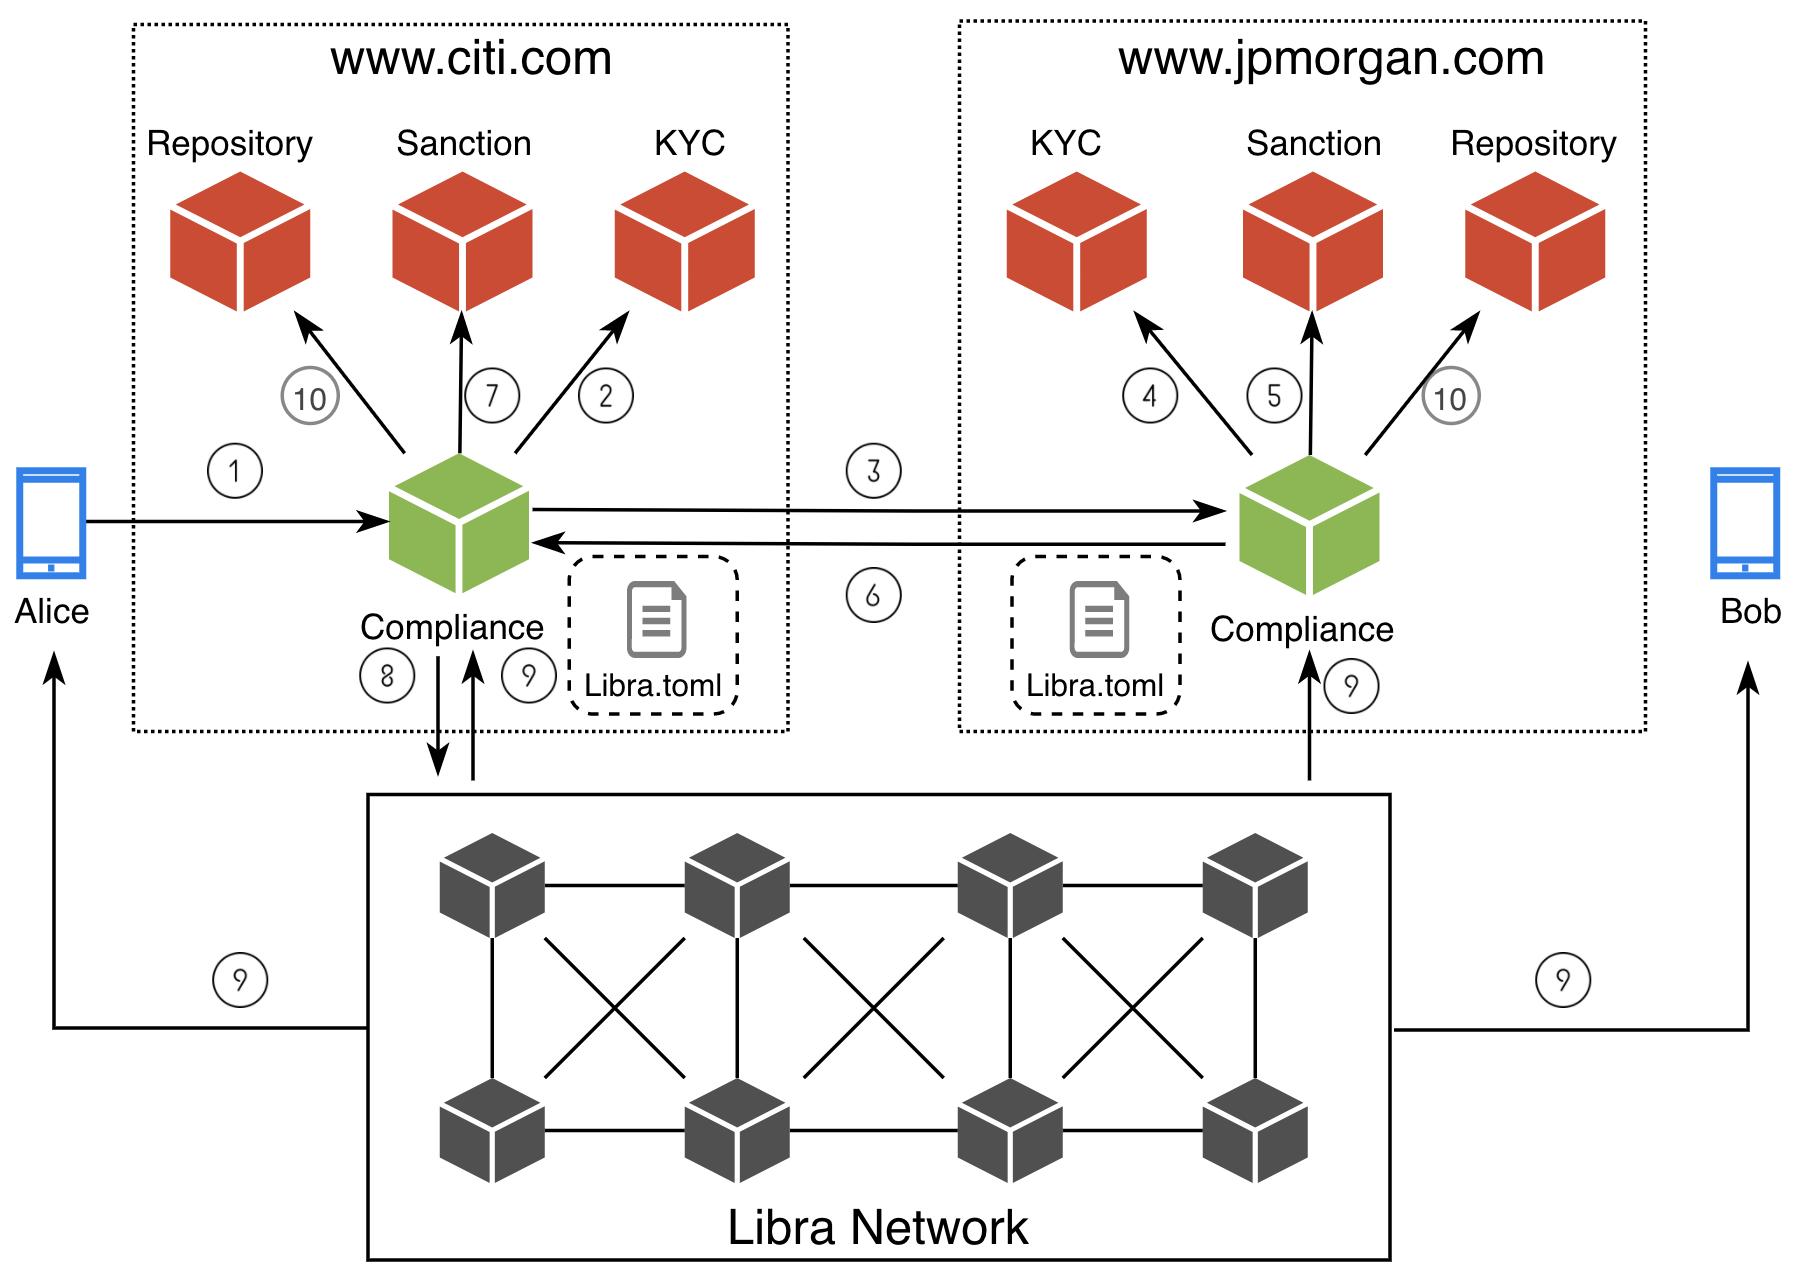
\includegraphics[width=12cm, keepaspectratio]{images/compliance.png}
    \caption{合规审核流程}
    \label{fig:compliance}
\end{figure}
\begin{enumerate}
    \item Alice 获取 Bob 的身份账户与资产账户,构建一个交易请求并且签名。Alice 通过花旗银行的 libra.toml 文件获取合规服务的URL,将签名后的交易提交给花旗银行的合规服务处理。
    
    \begin{lstlisting}[caption={Alice 请求花旗银行审核交易}, label={lst:alice_request}]
    POST https://www.citi.com/aml/newTx      HTTP/1.1
    Content-Type:   application/json
    {
        "data": {
            "sender": "<Alice's identity account>",
            "recipiant": "<Bob's identity account>",
            "tx": "<hex string of transaction signed with Alice's asset account>",
            "note": "<note about the transaction>"
        }
        "signature":"<Alice's signature of data field>"
    }
    \end{lstlisting}

    \item 花旗银行的合规服务收到 Alice 的请求之后,先查询本地的 KYC 服务,确认 Alice 的身份信息。

    \item 花旗银行解析 Bob 的身份账户数据,判定接收方的合规机构是摩根银行。然后找到摩根银行的合规服务URL。将 Alice 的交易与 KYC 数据打包,请求摩根银行根据 Alice 和 Bob 的KYC数据审核该交易是否受AML制裁限制,同时也请求返回 Bob 的KYC数据。

    \begin{lstlisting}[caption={花旗银行请求摩根银行审核交易}, label={lst:citi_request}]
    POST https://www.jpmorgan.com/aml/sanctionCheck      HTTP/1.1
    Content-Type:   application/json
    {
        "data": {
            "sender": "<Alice's account>",
            "need_recipiant_info": "Yes",
            "tx": "<hex string of transaction signed with Alice's asset account>",
            "attachment": {
                "nonce": "<nounce>",
                "sender_info": {
                    "first_name": "<Alice's first_name>",
                    "middle_name": "<Alice's middle_name>",
                    "last_name": "<Alice's last_name>",
                    "address": "<Alice's address>",
                    "city": "<Alice's city>",
                    "province": "<Alice's province>",
                    "country": "<Alice's nationality>",
                    "date_of_birth": "<Alice's birthday>",
                    "company_name": "<Alice's company name>"
                },
                "note": "<note about the transaction>"
            }
        }
        "signature":"<the signature of data by Citi Bank>"
    }
    \end{lstlisting}

    \item 摩根银行的合规服务收到花旗的请求之后,先查询本地的 KYC 服务,确认 Bob 的身份信息。

    \item 摩根银行调用内部的 Sanction 子系统,审核此交易是否涉嫌洗钱。

    \item 如果通过AML制裁检查,摩根将审核的结果返回给花旗银行,并且将 Bob 的身份信息一并返回。

    \begin{lstlisting}[caption={摩根银行向花旗银行返回审核结果}, label={lst:jpm_reply}]
    HTTP/1.1 200 OK
    Content-Type:   application/json
    {
        "check_result": "ok",
        "info_result": "yes",
        "recipiant_info":{
            "first_name": "<Bob's first_name>",
            "middle_name": "<Bob's middle_name>",
            "last_name": "<Bob's last_name>",
            "address": "<Bob's address>",
            "city": "<Bob's city>",
            "province": "<Bob's province>",
            "country": "<Bob's nationality>",
            "date_of_birth": "<Bob's birthday>",
            "company_name": "<Bob's company name>"
        }
        "signature":"<the signature of recipiant_info by JPM Bank>"
    }
    \end{lstlisting}

    \item 花旗银行获得 Bob 的身份信息后,与 Alice 的身份合并,根据本地的 Sanction 规则,重新审核此交易是否涉嫌洗钱。

    \item 如果花旗银行的AML制裁检查也通过,那么花旗银行对于此交易签名,广播到 Libra 网络上。所以此交易不仅仅包含 Alice 的签名,也包含花旗银行的签名。

    \item Libra 的矿工们收到未确认的交易,检查是否满足确认条件。验证的条件至少包括下列几项:
        \begin{itemize}
            \item   检查 花旗银行的签名,验证交易是否已经审核通过。
            \item   检查 Alice 的签名,验证其是否为发送账户的拥有者
            \item   检查 Alice 的资产账户余额是否充足等其它必要条件
        \end{itemize}
        以上条件都通过之后,所有矿工达成共识将此交易写入 Libra 账本。之后的全网同步过程中,Alice、Bob、花旗和摩根银行都会收到交易确认消息。

    \item 花旗和摩根银行将确认后的交易数据写入本地的 Trade Repository 归档,以备之后的审查。归档记录里面包含以下数据
        \begin{itemize}
            \item   发送方的相关信息: Alice 的身份信息、转出资产账户。
            \item   发送方合规机构的签名: 花旗银行的签名
            \item   接受方的相关信息: Bob 的身份信息、转入资产账户。
            \item   接受方合规机构的签名: 摩根银行的签名
            \item   交易的相关信息: 交易时间,额度等
        \end{itemize}
        这些归档数据可以向有关管理部门提供详尽、准确的历史数据,提高市场透明度,并支持相关公共政策目标。
\end{enumerate}

